\chapter{Specifikacija programske potpore}
		
	\section{Funkcionalni zahtjevi}			
			
			\noindent \textbf{Dionici:}
			
			\begin{packed_enum}
				
				\item Igrači
				\item Kartografi
				\item Administrator			
				\item Razvojni tim
				
			\end{packed_enum}
			
			\noindent \textbf{Aktori i njihovi funkcionalni zahtjevi:}
			
			
			\begin{packed_enum}
				\item  \underbar{Neregistrirani/neprijavljeni korisnik (inicijator) može:}
				
				\begin{packed_enum}
					
					\item obaviti registraciju:
						\begin{packed_enum}
							\item kao igrač  unosom korisničkog imena, fotografije, e-mail adrese i lozinke
							\item kao kartograf unosom korisničkog imena, fotografije, e-mail adrese, lozinke, IBAN-a te fotografije osobne iskaznice
						\end{packed_enum}
					\item ukoliko je korisnik već registriran u sustavu, mora se prijaviti koristeći korisničko ime ili e-mail adresu i lozinku
				\end{packed_enum}
			
				\item  \underbar{Igrač (inicijator) može:}
					
					\begin{packed_enum}
					
						\item pregledavati i mijenjati svoje korisničke podatke
						\item izbrisati svoj korisnički račun
						\item vidjeti kartu na kojoj su označene lokacije na kojima se mogu skupiti karte te njegova lokacija
						\item vidjeti informacije o lokacijama (naziv, opis, fotografiju, kategoriju i jačinu karte te lokacije)
						\item vidjeti kolekciju svojih karata
						\item vidjeti popis ostalih aktivnih igrača koji se nalaze u krugu od 50km i s njima ući u borbu
						\item prijaviti novu lokaciju
						\item vidjeti globalnu statistiku odigranih borbi i sakupljenih lokacija
						\item vidjeti poredak svih igrača
						\item vidjeti profil drugog igrača (njegove karte, rang na globalnoj ljestvici i statistike vezane uz zadnjih 10 borbi s drugim igračima)
					
					\end{packed_enum}
				
				\item  \underbar{Kartograf (inicijator) može:}
				
				\begin{packed_enum}
					
					\item vidjeti kartu sa:
					\begin{packed_enum}
						
						\item prijavljenim lokacijama za unos u bazu podataka
						\item prikazanim najkraćim putem do lokacije koju treba provjeriti na terenu
						\item već unesenim lokacijama u bazi podataka
					
					\end{packed_enum}
					
					\item odbiti, potvrditi, urediti ili označiti da je potrebna potvrda s terena za prijavljenu lokaciju
					\item dodavati lokacije u bazu podataka
					\item vidjeti i izmjeniti svoje osobne podatke
					
				\end{packed_enum}
			
				\item  \underbar{Administrator (inicijator) može:}
				
				\begin{packed_enum}
					
					\item vidjeti i uređivati popis svih korisnika i njihovih osobnih podataka
					\item dodjeliti igračima privremeno isključenje iz igre
					\item vidjeti i uređivati postojeće lokacije
					\item vidjeti globalnu statistiku odigranih borbi i sakupljenih lokacija
					\item vidjeti poredak svih igrača
					
				\end{packed_enum}
			
				\item  \underbar{Baza podataka (sudionik):}
				
				\begin{packed_enum}
					
					\item pohranjuje sve podatke o korisnicima i njihovim ovlastima
					\item  pohranjuje sve podatke o kartama i lokacijama
					\item  pohranjuje sve podatke o borbama i rang listama igrača
					
				\end{packed_enum}
			\end{packed_enum}
			
			\eject 
			
			
				
			\subsection{Obrasci uporabe}
		
				\subsubsection{Opis obrazaca uporabe}
				
					\noindent \underbar{\textbf{UC1 - Početni zaslon za neprijavljenog korisnika}}
					\begin{packed_item}
						
						\item \textbf{Glavni sudionik: }Korisnik
						\item  \textbf{Cilj:} Prikaz početnog zaslona za neprijavljenog korisnika
						\item  \textbf{Sudionici:} Baza podataka
						\item  \textbf{Preduvjet:} -
						\item  \textbf{Opis osnovnog tijeka:}
						
						\item[] \begin{packed_enum}
							
							\item Korisnik pristupa aplikaciji
							\item Otvara se početni zaslon za neprijavljenog korisnika
						\end{packed_enum}
					\end{packed_item}
					
					
					\noindent \underbar{\textbf{UC2 -Registracija igrača}}
					\begin{packed_item}
	
						\item \textbf{Glavni sudionik: }Korisnik
						\item  \textbf{Cilj:} Stvoriti korisnički račun za pristup sustavu
						\item  \textbf{Sudionici:} Baza podataka
						\item  \textbf{Preduvjet:} -
						\item  \textbf{Opis osnovnog tijeka:}
						
						\item[] \begin{packed_enum}
	
							\item Korisnik odabire opciju za registraciju igrača
							\item Korisnik unosi potrebne korisničke podatke(korisničko ime, e-mail, lozinka)
							\item Korisnik prima obavijest o uspješnoj registraciji
							\item Nakon registracije korisnik automatski prijavljen u sustav
						\end{packed_enum}
						
						\item  \textbf{Opis mogućih odstupanja:}
						
						\item[] \begin{packed_item}
	
							\item[2.a] Odabir već zauzetog korisničkog imena i/ili e-maila ili pružanje neispravnog e-maila
							\item[] \begin{packed_enum}
								
								\item Sustav obavještava korisnika o neuspjelom upisu i vraća ga na stranicu za registraciju 
								\item Korisnik mijenja potrebne podatke te završava unos ili odustaje od registracije
								
							\end{packed_enum}
							\item[2.b] Odabir "slabe" lozinke(za "jaku" lozinku obavezno barem 8 znakova, 1 veliko slovo, 1 broj)
							\item[] \begin{packed_enum}
								\item Sustav obavještava korisnika da je lozinka "slaba" i vraća ga na stranicu za registraciju
								\item Korisnik odabire "jaču" lozinku te završava unos ili odustaje od registracije 
								
							\end{packed_enum}
								
						\end{packed_item}
					\end{packed_item}
				
					\noindent \underbar{\textbf{UC3 - Registracija katografa}}
					\begin{packed_item}
						
						\item \textbf{Glavni sudionik: }Kartograf
						\item  \textbf{Cilj:} Stvoriti korisnički račun za kartografa
						\item  \textbf{Sudionici:} Baza podataka
						\item  \textbf{Preduvjet:} -
						\item  \textbf{Opis osnovnog tijeka:}
						
						\item[] \begin{packed_enum}
							
							\item Korisnik odabire opciju za registraciju kartografa
							\item Korisnik unosi potrebne korisničke podatke(korisničko ime, e-mail, lozinka)
							\item Korisnik prima obavijest o uspješnoj registraciji
						\end{packed_enum}
						
						\item  \textbf{Opis mogućih odstupanja:}
						
						\item[] \begin{packed_item}
							
							\item[2.a] Odabir već zauzetog korisničkog imena i/ili e-maila ili pružanje neispravnog e-maila
							\item[] \begin{packed_enum}
								
								\item Sustav obavještava korisnika o neuspjelom upisu i vraća ga na stranicu za registraciju kartografa
								\item Korisnik mijenja potrebne podatke te završava unos ili odustaje od registracije
								
							\end{packed_enum}
							\item[2.b] Odabir "slabe" lozinke(za "jaku" lozinku obavezno barem 8 znakova, 1 veliko slovo, 1 broj)
							\item[] \begin{packed_enum}
								\item Sustav obavještava korisnika da je lozinka "slaba" i vraća ga na stranicu za registraciju
								\item Korisnik odabire "jaču" lozinku te završava unos ili odustaje od registracije 
								
							\end{packed_enum}
							
						\end{packed_item}
					\end{packed_item}
					
				
					\noindent \underbar{\textbf{UC4 -Prijava u sustav}}
					\begin{packed_item}
					
					\item \textbf{Glavni sudionik: }Igrač
					\item  \textbf{Cilj:} Dobiti pristup korisničkom sučelju
					\item  \textbf{Sudionici:} Baza podataka
					\item  \textbf{Preduvjet:} Registracija
					\item  \textbf{Opis osnovnog tijeka:}
					
					\item[] \begin{packed_enum}
						
						\item Unos korisničkog imena ili e-maila i lozinke
						\item Potvrda o ispravnosti unesenih podataka
						\item Pristup korisničkim funkcijama
					\end{packed_enum}
					
					\item  \textbf{Opis mogućih odstupanja:}
					
					\item[] \begin{packed_item}
						
						\item[2.a] Unos neispravnog korisničkog imena, e-maila ili lozinke
						\item[] \begin{packed_enum}
							
							\item Sustav obavještava korisnika o neispravnom upisu i vraća ga na stranicu za prijavu
							
						\end{packed_enum}
						
					\end{packed_item}
					\end{packed_item}
				
					\noindent \underbar{\textbf{UC5 - Pregled lokacija na karti}}
					\begin{packed_item}
						
						\item \textbf{Glavni sudionik: }Igrač
						\item  \textbf{Cilj:} Pregled lokacija koje igrač može posjetiti
						\item  \textbf{Sudionici:} Baza podataka
						\item  \textbf{Preduvjet:} Igrač je prijavljen
						\item  \textbf{Opis osnovnog tijeka:}
						
						\item[] \begin{packed_enum}
							
							\item Korisnik odabire opciju pregled lokacija na karti
							\item Otvara karta s lokacijama
						\end{packed_enum}
					\end{packed_item}
					
					\noindent \underbar{\textbf{UC6 -Pregled informacija o lokaciji}}
					\begin{packed_item}
						
						\item \textbf{Glavni sudionik: }Igrač
						\item  \textbf{Cilj:} Pregled informacija o lokaciji
						\item  \textbf{Sudionici:} Baza podataka
						\item  \textbf{Preduvjet:} Igrač je prijavljen
						\item  \textbf{Opis osnovnog tijeka:}
						
						\item[] \begin{packed_enum}
							
							\item Korisnik odabire opciju "Informacija o lokaciji"
							\item Aplikacija prikazuje informacije o lokaciji
						\end{packed_enum}
					\end{packed_item}
					
					
					\noindent \underbar{\textbf{UC7 -Pregled osobnih podataka igrača}}
					\begin{packed_item}
					
					\item \textbf{Glavni sudionik: }Igrač
					\item  \textbf{Cilj:} Pregledati osobne podatke
					\item  \textbf{Sudionici:} Baza podataka
					\item  \textbf{Preduvjet:} Igrač je prijavljen
					\item  \textbf{Opis osnovnog tijeka:}
					
					\item[] \begin{packed_enum}
						
						\item Korisnik odabire opciju "Osobni podatci"
						\item Aplikacija prikazuje osobne podatke korisnika
					\end{packed_enum}
					\end{packed_item}
			
					\noindent \underbar{\textbf{UC8 -Promjena osobnih podataka igrača}}
					\begin{packed_item}
					
					\item \textbf{Glavni sudionik: }Igrač
					\item  \textbf{Cilj:} Promjeniti osobne podatke
					\item  \textbf{Sudionici:} Baza podataka
					\item  \textbf{Preduvjet:} Igrač je prijavljen
					\item  \textbf{Opis osnovnog tijeka:}
					
					\item[] \begin{packed_enum}
						
						\item Korisnik odabire opciju za promjenu podataka
						\item Korisnik mijenja svoje osobne podatke
						\item Korisnik sprema promjene
						\item Baza podataka se ažurira
					\end{packed_enum}
					
					\item  \textbf{Opis mogućih odstupanja:}
					
					\item[] \begin{packed_item}
						
						\item[2.a] Odabir već zauzetog korisničkog imena i/ili e-maila
						\item[] \begin{packed_enum}
							
							\item Sustav obavještava korisnika da je korisničko ime i/ili e-mail već zauzeto i traži ponovni unos
							\item Korisnik unosi novo korisničko ime i/ili e-maila ili odustaje je promjene osobnih podataka
							
						\end{packed_enum}
						\item[2.b] Korisnik odabire "slabu" zamjensku lozinku
						\item[] \begin{packed_enum}
							\item Sustav obavještava korisnika da je odabrao "slabu" lozinku i traži ponovni unos
							\item Korisnik unosi novu lozinku koja je dovoljno "jaka" ili odustaje od promjene lozinke
						\end{packed_enum}
						\item[2.c] Korisnik promijeni svoje osobne podatke, ali ne odabere opciju "Spremi promjenu"
						\item[] \begin{packed_enum}
							\item Sustav obavještava korisnika da nije spremio podatke prije izlaska iz prozora
						\end{packed_enum}
						
					\end{packed_item}
					\end{packed_item}
				
					\noindent \underbar{\textbf{UC9 - Pregled osobnih podataka kartografa}}
					\begin{packed_item}
						
						\item \textbf{Glavni sudionik: }Kartograf
						\item  \textbf{Cilj:} Pregledati osobne podatke
						\item  \textbf{Sudionici:} Baza podataka
						\item  \textbf{Preduvjet:} Kartograf je prijavljen
						\item  \textbf{Opis osnovnog tijeka:}
						
						\item[] \begin{packed_enum}
							
							\item Korisnik odabire opciju "Osobni podatci"
							\item Aplikacija prikazuje osobne podatke korisnika
						\end{packed_enum}
					\end{packed_item}
					
					\noindent \underbar{\textbf{UC10 -Promjena osobnih podataka kartografa}}
					\begin{packed_item}
						
						\item \textbf{Glavni sudionik: }Kartograf
						\item  \textbf{Cilj:} Promjeniti osobne podatke
						\item  \textbf{Sudionici:} Baza podataka
						\item  \textbf{Preduvjet:} Kartograf je prijavljen
						\item  \textbf{Opis osnovnog tijeka:}
						
						\item[] \begin{packed_enum}
							
							\item Korisnik odabire opciju za promjenu podataka
							\item Korisnik mijenja svoje osobne podatke
							\item Korisnik sprema promjene
							\item Baza podataka se ažurira
						\end{packed_enum}
						
						\item  \textbf{Opis mogućih odstupanja:}
						
						\item[] \begin{packed_item}
							
							\item[2.a] Odabir već zauzetog korisničkog imena i/ili e-maila
							\item[] \begin{packed_enum}
								
								\item Sustav obavještava korisnika da je korisničko ime i/ili e-mail već zauzeto i traži ponovni unos
								\item Korisnik unosi novo korisničko ime i/ili e-maila ili odustaje je promjene osobnih podataka
								
							\end{packed_enum}
							\item[2.b] Korisnik odabire "slabu" zamjensku lozinku
							\item[] \begin{packed_enum}
								\item Sustav obavještava korisnika da je odabrao "slabu" lozinku i traži ponovni unos
								\item Korisnik unosi novu lozinku koja je dovoljno "jaka" ili odustaje od promjene lozinke
							\end{packed_enum}
							\item[2.c] Korisnik promijeni svoje osobne podatke, ali ne odabere opciju "Spremi promjenu"
							\item[] \begin{packed_enum}
								\item Sustav obavještava korisnika da nije spremio podatke prije izlaska iz prozora
							\end{packed_enum}
							
						\end{packed_item}
					\end{packed_item}
					
					\noindent \underbar{\textbf{UC5 -Brisanje korisničkog računa}}
					\begin{packed_item}
						
						\item \textbf{Glavni sudionik: }Igrač, kartograf
						\item  \textbf{Cilj:} Izbrisati svoj korisnički račun
						\item  \textbf{Sudionici:} Baza podataka
						\item  \textbf{Preduvjet:} Igrač je prijavljen
						\item  \textbf{Opis osnovnog tijeka:}
						
						\item[] \begin{packed_enum}
							
							\item Korisnik otvara stranicu s osobnim podacima
							\item Korisnik briše račun
							\item Sustav traži potvrdu brisanja korisničkog računa
							\item Korisnik odobrava brisanje
							\item Korisnički račun se izbriše iz baze podataka
							\item Otvara se stranica za registraciju
						\end{packed_enum}
						
					\end{packed_item}
				
					\noindent \underbar{\textbf{UC12 -Pregled (vlastith) sakupljenih karata}}
					\begin{packed_item}
						
						\item \textbf{Glavni sudionik: }Igrač, administrator
						\item  \textbf{Cilj:} Pregled skupljenih karata igrača
						\item  \textbf{Sudionici:} Baza podataka
						\item  \textbf{Preduvjet:} Igrač je prijavljen i skupio barem jednu kartu
						\item  \textbf{Opis osnovnog tijeka:}
						
						\item[] \begin{packed_enum}
							
							\item Korisnik odabire opciju za pregled skupljenih karata
							\item Otvara se stranica sa skupljenim kartama korisnika
						\end{packed_enum}
						
						\item  \textbf{Opis mogućih odstupanja:}
						
						\item[] \begin{packed_item}
							
							\item[2.a] Korisnik nije skupio niti jednu kartu
							\item[] \begin{packed_enum}
								
								\item Sustav obavještava korisnika da mora skupiti barem jednu kartu da moze pristupiti pregledu i vraća ga na kartu
								
							\end{packed_enum}
						\end{packed_item}
					\end{packed_item}
				
					\noindent \underbar{\textbf{UC13 -Pregled vlastite statistike igrača}}
					\begin{packed_item}
						
						\item \textbf{Glavni sudionik: }Igrač
						\item  \textbf{Cilj:} Pregledati vlastitu statistiku
						\item  \textbf{Sudionici:} Baza podataka
						\item  \textbf{Preduvjet:} Igrač je prijavljen
						\item  \textbf{Opis osnovnog tijeka:}
						
						\item[] \begin{packed_enum}
							
							\item Korisnik odabire opciju "Moja statistika"
							\item Aplikacija prikazuje vlastitu statistiku igrača
						\end{packed_enum}
					\end{packed_item}
					
					\noindent \underbar{\textbf{UC14 - Pregled (vlastith) odigranih borbi}}
					\begin{packed_item}
						
						\item \textbf{Glavni sudionik: }Igrač
						\item  \textbf{Cilj:} Pregled borbi u kojima je igrač sudjelovao
						\item  \textbf{Sudionici:} Baza podataka
						\item  \textbf{Preduvjet:} Igrač je prijavljen i odigrao barem jednu borbu
						\item  \textbf{Opis osnovnog tijeka:}
						
						\item[] \begin{packed_enum}
							
							\item Korisnik odabire opciju za pregled odigranih borbi
							\item Otvara se stranica s odigranim borbama
						\end{packed_enum}
						
						\item  \textbf{Opis mogućih odstupanja:}
						
						\item[] \begin{packed_item}
							
							\item[2.a] Korisnik nije sudjelovao u niti jednoj borbi
							\item[] \begin{packed_enum}
								
								\item Sustav obavještava korisnika da nije sudjelovao u brobi
							\end{packed_enum}
						\end{packed_item}
					\end{packed_item}
					
					\noindent \underbar{\textbf{UC15 -Pregled vlastite statistike kartografa}}
					\begin{packed_item}
						
						\item \textbf{Glavni sudionik: }Kartograf
						\item  \textbf{Cilj:} Pregledati vlastitu statistiku
						\item  \textbf{Sudionici:} Baza podataka
						\item  \textbf{Preduvjet:} Kartograf je prijavljen
						\item  \textbf{Opis osnovnog tijeka:}
						
						\item[] \begin{packed_enum}
							
							\item Korisnik odabire opciju "Moja statistika"
							\item Aplikacija prikazuje vlastitu statistiku kartografa
						\end{packed_enum}
					\end{packed_item}
					
					\noindent \underbar{\textbf{UC16 - Pregled profila ostalih igrača}}
					\begin{packed_item}
						
						\item \textbf{Glavni sudionik: }Igrač
						\item  \textbf{Cilj:} Pregled profila ostalih igrača
						\item  \textbf{Sudionici:} Baza podataka
						\item  \textbf{Preduvjet:} Igrač je prijavljen
						\item  \textbf{Opis osnovnog tijeka:}
						
						\item[] \begin{packed_enum}
							
							\item Korisnik odabire profil drugog igrača
							\item Otvara se profil drugog igrača
						\end{packed_enum}
					\end{packed_item}
					
					\noindent \underbar{\textbf{UC17 -Pregled statistike ostalih igrača}}
					\begin{packed_item}
						
						\item \textbf{Glavni sudionik: }Igrač
						\item  \textbf{Cilj:} Pregledati statistiku ostalih igrača
						\item  \textbf{Sudionici:} Baza podataka
						\item  \textbf{Preduvjet:} Igrač je prijavljen
						\item  \textbf{Opis osnovnog tijeka:}
						
						\item[] \begin{packed_enum}
							
							\item Korisnik odabire opciju "Statistika"
							\item Aplikacija prikazuje statistiku igrača
						\end{packed_enum}
					\end{packed_item}
					
					\noindent \underbar{\textbf{UC18 -Pregled sakupljenih karata ostalih igrača}}
					\begin{packed_item}
						
						\item \textbf{Glavni sudionik: }Igrač
						\item  \textbf{Cilj:} Pregled skupljenih karata igrača
						\item  \textbf{Sudionici:} Baza podataka
						\item  \textbf{Preduvjet:} Igrač je prijavljen i skupio barem jednu kartu
						\item  \textbf{Opis osnovnog tijeka:}
						
						\item[] \begin{packed_enum}
							
							\item Korisnik odabire opciju za pregled skupljenih karata
							\item Otvara se stranica sa skupljenim kartama korisnika
						\end{packed_enum}
						
						\item  \textbf{Opis mogućih odstupanja:}
						
						\item[] \begin{packed_item}
							
							\item[2.a] Korisnik nije skupio niti jednu kartu
							\item[] \begin{packed_enum}
								
								\item Sustav obavještava korisnika da igrač nije sakupio niti jednu kartu			
							\end{packed_enum}
						\end{packed_item}
					\end{packed_item}
				
					\noindent \underbar{\textbf{UC19 - Izazivanje na borbu igrača u blizini}}
					\begin{packed_item}
						
						\item \textbf{Glavni sudionik: }Igrač
						\item  \textbf{Cilj:} Izazvati ostale igrače na borbu
						\item  \textbf{Sudionici:} Baza podataka
						\item  \textbf{Preduvjet:} Igrač je prijavljen i sakupio barem tri karte
						\item  \textbf{Opis osnovnog tijeka:}
						
						\item[] \begin{packed_enum}
							
							\item Korisnik odabire opciju "Izazovi"
							\item Otvara se stranica za borbu igrača
						\end{packed_enum}
						
						\item  \textbf{Opis mogućih odstupanja:}
						
						\item[] \begin{packed_item}
							
							\item[2.a] Korisnik nije skupio barem tri karte
							\item[] \begin{packed_enum}
								
								\item Sustav obavještava korisnika da mora skupiti barem tri kartu da moze sudjelovati u borbi
								
							\end{packed_enum}
						\end{packed_item}
					\end{packed_item}
					
					\noindent \underbar{\textbf{UC20 - Odluka o prihvaćanju izazova}}
					\begin{packed_item}
						
						\item \textbf{Glavni sudionik: }Igrač
						\item  \textbf{Cilj:} Igrač može prihvatiti ili odbiti borbu
						\item  \textbf{Sudionici:} Baza podataka
						\item  \textbf{Preduvjet:} Igrač je prijavljen i sakupio barem tri karte
						\item  \textbf{Opis osnovnog tijeka:}
						
						\item[] \begin{packed_enum}
							
							\item Korisnik odabire opciju za prihvaćanje izazova ili odbijanje
						\end{packed_enum}
						
						\item  \textbf{Opis mogućih odstupanja:}
						
						\item[] \begin{packed_item}
							
							\item[2.a] Korisnik nije skupio barem tri karte
							\item[] \begin{packed_enum}
								
								\item Sustav obavještava korisnika da mora skupiti barem tri kartu da može sudjelovati u borbi
								\item Borba se odbija
								
							\end{packed_enum}
						\end{packed_item}
					\end{packed_item}
					
					\noindent \underbar{\textbf{UC21 - Borba igrača}}
					\begin{packed_item}
						
						\item \textbf{Glavni sudionik: }Igrač
						\item  \textbf{Cilj:} Borba igrača za najbolji globalni rang
						\item  \textbf{Sudionici:} Baza podataka
						\item  \textbf{Preduvjet:} Igrač je prijavljen
						\item  \textbf{Opis osnovnog tijeka:}
						
						\item[] \begin{packed_enum}
							
							\item Korisnik odabire igrača s kojim se želi boriti
							\item Izazvani igrač prihvaća ili odbija borbu
							\item Ako je igrač prihvatio borbu, borba počinje
						\end{packed_enum}
					\end{packed_item}
				
					\noindent \underbar{\textbf{UC22 - Pregled globalnog ranga igrača}}
					\begin{packed_item}
						
						\item \textbf{Glavni sudionik: }Igrač
						\item  \textbf{Cilj:} Pregled globalnog ranga igrača
						\item  \textbf{Sudionici:} Baza podataka
						\item  \textbf{Preduvjet:} Igrač je prijavljen
						\item  \textbf{Opis osnovnog tijeka:}
						
						\item[] \begin{packed_enum}
							
							\item Korisnik odabire opciju za pregled globalnog ranga igrača
							\item Otvara se stranica s globalnim rangom igrača
						\end{packed_enum}
					\end{packed_item}
				
					\noindent \underbar{\textbf{UC23 - Globalna statistika odigranih borbi}}
					\begin{packed_item}
						
						\item \textbf{Glavni sudionik: }Igrač
						\item  \textbf{Cilj:} Globalna statistika odigranih borbi
						\item  \textbf{Sudionici:} Baza podataka
						\item  \textbf{Preduvjet:} Igrač je prijavljen
						\item  \textbf{Opis osnovnog tijeka:}
						
						\item[] \begin{packed_enum}
							
							\item Korisnik odabire opciju za pregled globalne statistike odigranih borbi
							\item Otvara se stranica globalnom statistikom odigranih borbi
						\end{packed_enum}
					\end{packed_item}
					
					\noindent \underbar{\textbf{UC24 - Globalna statistika sakupljenih lokacija}}
					\begin{packed_item}
						
						\item \textbf{Glavni sudionik: }Igrač
						\item  \textbf{Cilj:} Globalna statistika sakupljenih lokacija
						\item  \textbf{Sudionici:} Baza podataka
						\item  \textbf{Preduvjet:} Igrač je prijavljen
						\item  \textbf{Opis osnovnog tijeka:}
						
						\item[] \begin{packed_enum}
							
							\item Korisnik odabire opciju za pregled globalne statistike sakupljenih lokacija
							\item Otvara se stranica globalnom statistikom sakupljenih lokacija
						\end{packed_enum}
					\end{packed_item}
					
					\noindent \underbar{\textbf{UC25 - Prijava nove lokacije}}
					\begin{packed_item}
						
						\item \textbf{Glavni sudionik: }Igrač
						\item  \textbf{Cilj:} Dodati novu lokaciju
						\item  \textbf{Sudionici:} Baza podataka
						\item  \textbf{Preduvjet:} Igrač je prijavljen
						\item  \textbf{Opis osnovnog tijeka:}
						
						\item[] \begin{packed_enum}
							
							\item Korisnik odabire lokaciju koju želi dodati
							\item Korisnik dodaje karakteristike lokacije
						\end{packed_enum}
					\end{packed_item}
				
					\noindent \underbar{\textbf{UC26 - Verificiranje prijavljene lokacije}}
					\begin{packed_item}
						
						\item \textbf{Glavni sudionik: }Kartograf
						\item  \textbf{Cilj:} Verificirati prijavljenu lokaciju
						\item  \textbf{Sudionici:} Baza podataka
						\item  \textbf{Preduvjet:} Kartograf je prijavljen
						\item  \textbf{Opis osnovnog tijeka:}
						
						\item[] \begin{packed_enum}
							
							\item Kartograf potvrđuje ispravnost lokacije
							\item Baza podataka se ažurira
						\end{packed_enum}
					\end{packed_item}
					
				
					\noindent \underbar{\textbf{UC27 - Brisanje lokacije}}
					\begin{packed_item}
						
						\item \textbf{Glavni sudionik: }Kartograf, administrator
						\item  \textbf{Cilj:} Obrisati nepostojeću/neispravnu lokaciju
						\item  \textbf{Sudionici:} Baza podataka
						\item  \textbf{Preduvjet:} -
						\item  \textbf{Opis osnovnog tijeka:}
						
						\item[] \begin{packed_enum}
							
							\item Kartograf/administrator odabire lokaciju koju želi obrisati
							\item Baza podataka se ažurira
						\end{packed_enum}
					\end{packed_item}
				
					\noindent \underbar{\textbf{UC28 - Pregled svih prijavljenih(neobrađenih) lokacija}}
					\begin{packed_item}
						
						\item \textbf{Glavni sudionik: }Kartograf
						\item  \textbf{Cilj:} Pregled prijavljenih lokacija koje nisu obrađene
						\item  \textbf{Sudionici:} Baza podataka
						\item  \textbf{Preduvjet:} Kartograf je prijavljen
						\item  \textbf{Opis osnovnog tijeka:}
						
						\item[] \begin{packed_enum}
							
							\item Korisnik odabire opciju pregled svih prijavljenih lokacija
							\item Otvara se popis svih prijavljenih lokacija koje nisu obrađene
						\end{packed_enum}
					\end{packed_item}
					
					\noindent \underbar{\textbf{UC29 - Karta s prikazanim najkraćim putem do lokacije za provjeru}}
					\begin{packed_item}
						
						\item \textbf{Glavni sudionik: }Kartograf
						\item  \textbf{Cilj:} Prikaz karte s s prikazanim najkraćim putem do lokacije za provjeru
						\item  \textbf{Sudionici:} Baza podataka
						\item  \textbf{Preduvjet:} Kartograf je prijavljen
						\item  \textbf{Opis osnovnog tijeka:}
						
						\item[] \begin{packed_enum}
							
							\item Korisnik odabire opciju karta s prikazanim najkraćim putem do lokacije za provjeru
							\item Otvara se karta
						\end{packed_enum}
					\end{packed_item}
					
				
					\noindent \underbar{\textbf{UC30 - Uređivanje postojeće lokacije}}
					\begin{packed_item}
						
						\item \textbf{Glavni sudionik: }Kartograf, administrator
						\item  \textbf{Cilj:} Promjeniti podatke o lokaciji
						\item  \textbf{Sudionici:} Baza podataka
						\item  \textbf{Preduvjet:} Kartograf je prijavljen
						\item  \textbf{Opis osnovnog tijeka:}
						
						\item[] \begin{packed_enum}
							
							\item Kartograf odabire lokaciju za koju želi promijeniti podatke
							\item Kartograf mijenja podatke
							\item Kartograf sprema promjene
							\item Baza podataka se ažurira
						\end{packed_enum}
						
						\item  \textbf{Opis mogućih odstupanja:}
						
						\item[] \begin{packed_item}
							
							\item[3.a] Kartograf promijeni podatke lokacije, ali ne odabere opciju "Spremi promjenu"
							\item[] \begin{packed_enum}
								\item Sustav obavještava kartografa da nije spremio podatke prije izlaska iz prozora
							\end{packed_enum}
						\end{packed_item}
					\end{packed_item}
				
					\noindent \underbar{\textbf{UC31 - Pregled svih odigranih borbi}}
					\begin{packed_item}
						
						\item \textbf{Glavni sudionik: }Administrator
						\item  \textbf{Cilj:} Pregled svih odigranih borbi
						\item  \textbf{Sudionici:} Baza podataka
						\item  \textbf{Preduvjet:} -
						\item  \textbf{Opis osnovnog tijeka:}
						
						\item[] \begin{packed_enum}
							
							\item Korisnik odabire opciju za pregled svih odigranih borbi
							\item Otvara se stranica s prikazom svih odigranih borbi
						\end{packed_enum}
					\end{packed_item}
					
					
					\noindent \underbar{\textbf{UC32 - Pregled korisnika}}
					\begin{packed_item}
						
						\item \textbf{Glavni sudionik: }Administrator
						\item  \textbf{Cilj:} Pregledati registrirane korisnike
						\item  \textbf{Sudionici:} Baza podataka
						\item  \textbf{Preduvjet:} Korisnik je prijavljen i dodijeljena su mu prava administratora
						\item  \textbf{Opis osnovnog tijeka:}
						
						\item[] \begin{packed_enum}
							
							\item Administrator odabire opciju pregledavanja korisnika
							\item Prikaže se lista svih ispravno registriranih korisnika s osobnim podacima
						\end{packed_enum}
					\end{packed_item}
				
					\noindent \underbar{\textbf{UC33 - Brisanje korisnika}}
					\begin{packed_item}
						
						\item \textbf{Glavni sudionik: }Administrator
						\item  \textbf{Cilj:} Obrisati korisnika
						\item  \textbf{Sudionici:} Baza podataka
						\item  \textbf{Preduvjet:} Korisnik je prijavljen i dodijeljena su mu prava administratora
						\item  \textbf{Opis osnovnog tijeka:}
						
						\item[] \begin{packed_enum}
							
							\item Administrator odabire opciju uklanjanja korisnika
							\item Administrator pronalazi željenog korisnika
							\item Administrator uklanja željenog korisnika i njegove podatke iz baze podataka
							\item Baza podataka se ažurira
						\end{packed_enum}
					\end{packed_item}
				
					\noindent \underbar{\textbf{UC34 - Promjena prava pristupa}}
					\begin{packed_item}
						
						\item \textbf{Glavni sudionik: }Administrator
						\item  \textbf{Cilj:} Promijeniti razinu pristupa korisnika (igrač, kartograf, administrator)
						\item  \textbf{Sudionici:} Baza podataka
						\item  \textbf{Preduvjet:} Korisnik je prijavljen i dodijeljena su mu prava administratora
						\item  \textbf{Opis osnovnog tijeka:}
						
						\item[] \begin{packed_enum}
							
							\item Administrator odabire opciju promjene prava pristupa
							\item Administrator pronalazi željenog korisnika
							\item Administrator mijenja razinu pristupa željenom korisniku
						\end{packed_enum}
					\end{packed_item}
				
					\noindent \underbar{\textbf{UC35 - Privremeno blokiranje korisnika}}
					\begin{packed_item}
						
						\item \textbf{Glavni sudionik: }Administrator
						\item  \textbf{Cilj:} Privremeno blokirati korisnika
						\item  \textbf{Sudionici:} Baza podataka
						\item  \textbf{Preduvjet:} Korisnik je prijavljen i dodijeljena su mu prava administratora
						\item  \textbf{Opis osnovnog tijeka:}
						
						\item[] \begin{packed_enum}
							
							\item Administrator odabire opciju privremenog blokiranja korisnika
							\item Administrator pronalazi željenog korisnika
							\item Administrator privremeno blokira željenog korisnika
						\end{packed_enum}
					\end{packed_item}
					
				\eject
					
				\subsubsection{Dijagrami obrazaca uporabe}
					
						%unos slike
					\begin{figure}[H]
						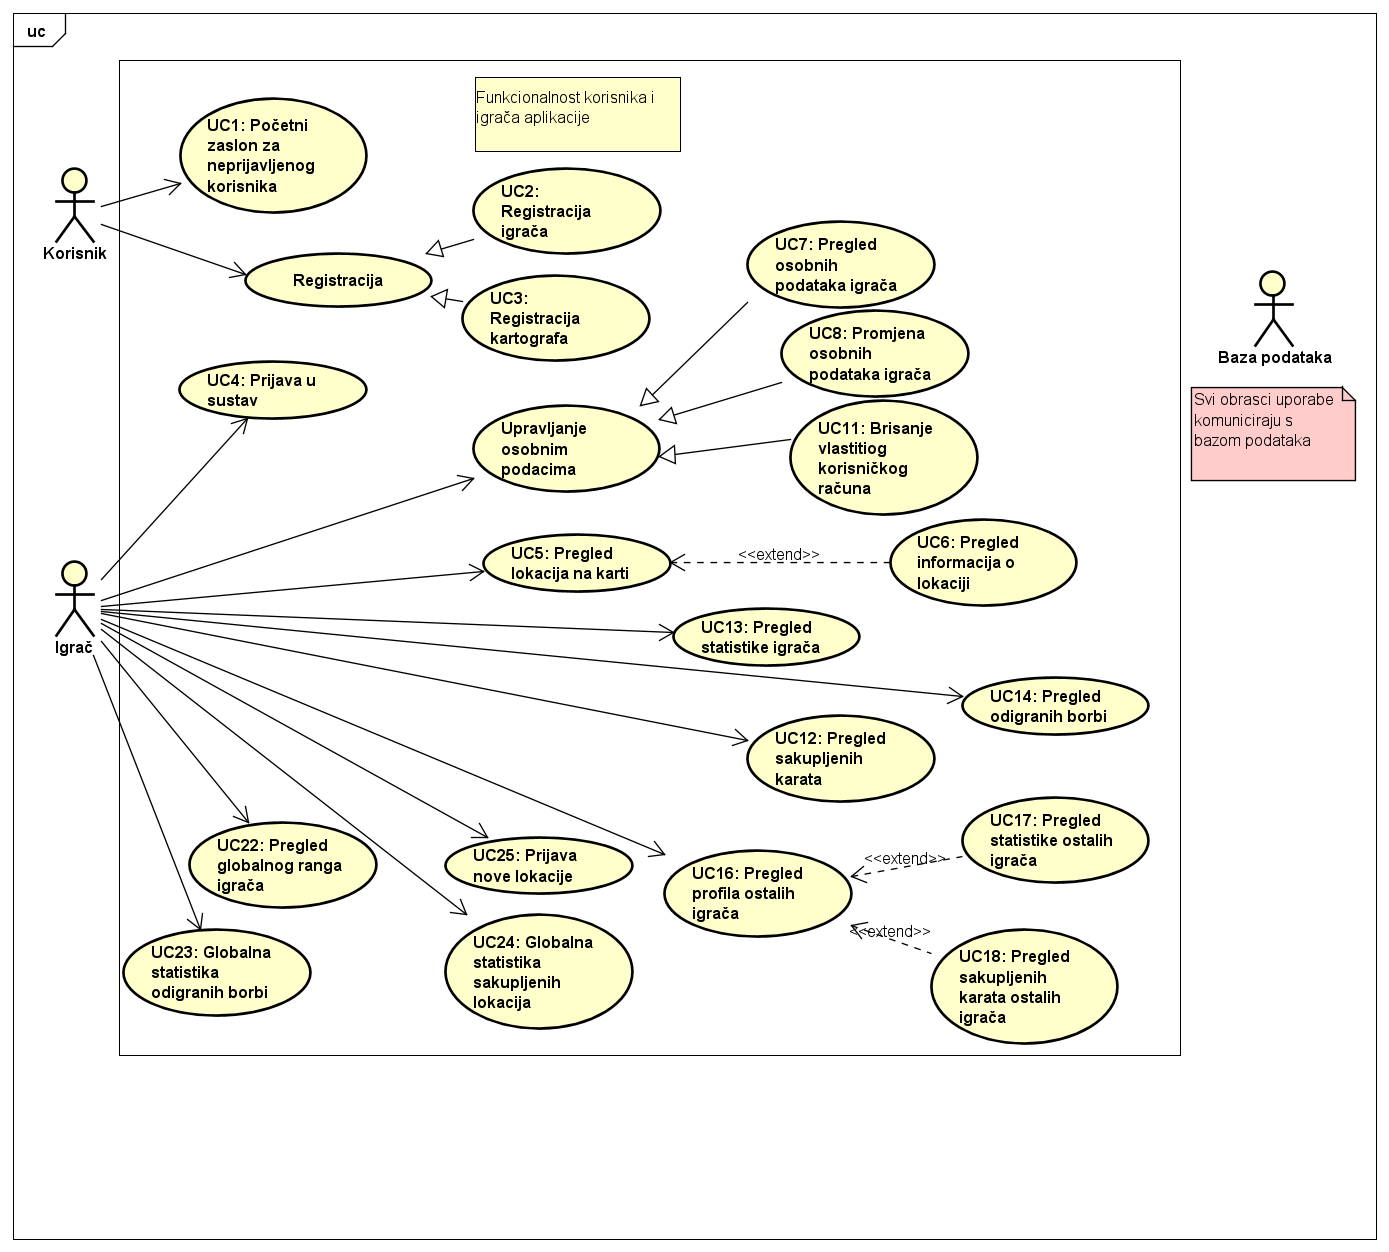
\includegraphics[width=\textwidth, height=16cm]{dijagrami/OU_igrac} 
						\centering
						\caption{Dijagram obrasca uporabe, funkcionalnost korisnika i klijenta}
						\label{}
					\end{figure}
					
					\begin{figure}[H]
						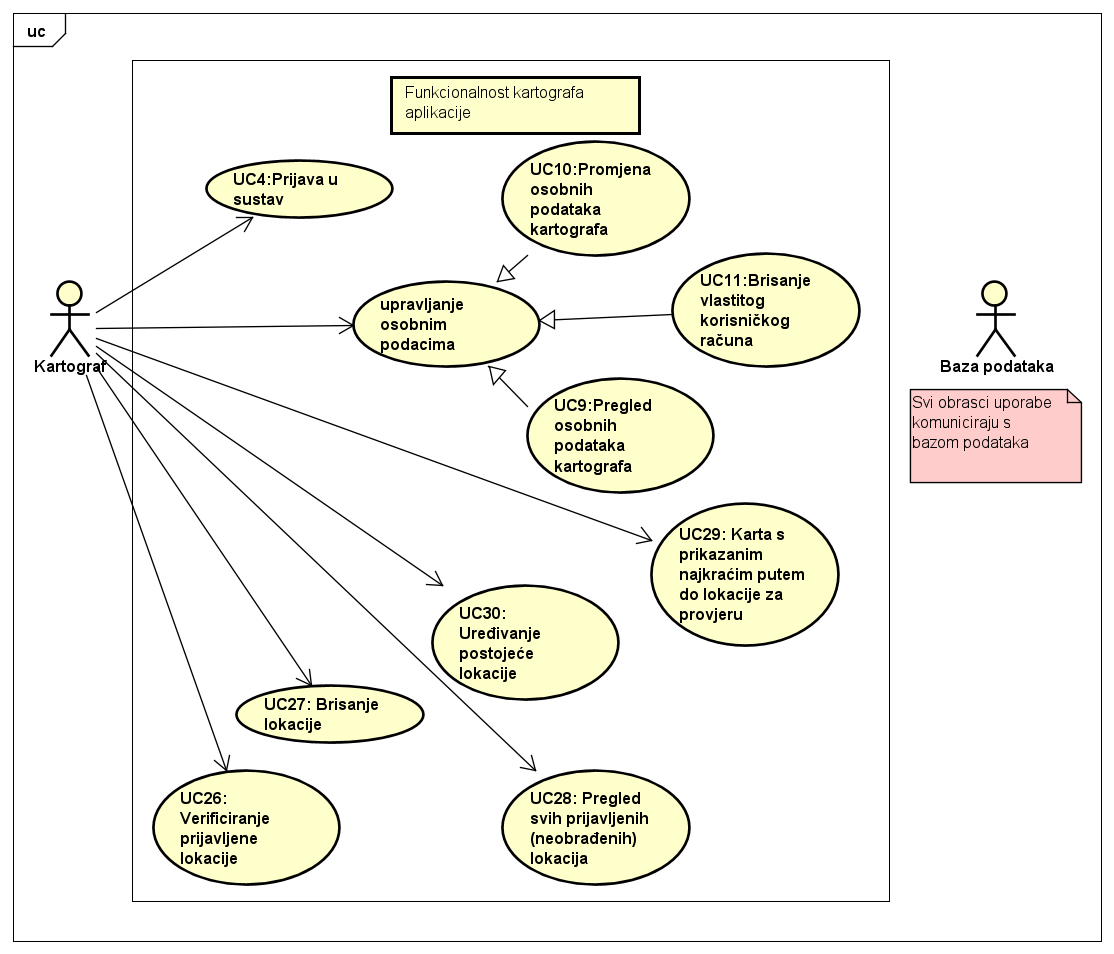
\includegraphics[width=\textwidth, height=14cm]{dijagrami/OU_kartograf}
						\centering
						\caption{Dijagram obrasca uporabe, funkcionalnost kartografa}
						\label{fig:promjene2} %label mora biti drugaciji za svaku sliku
					\end{figure}
				
					\begin{figure}[H]
						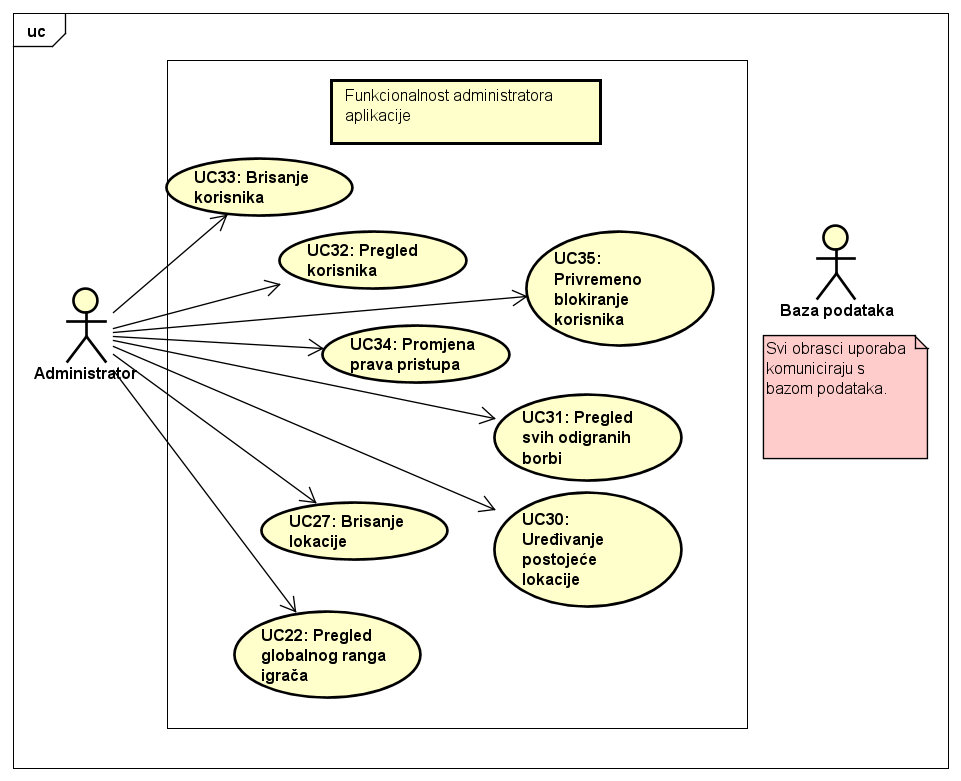
\includegraphics[width=\textwidth, height=12cm]{dijagrami/OU_admin} 
						\centering
						\caption{Dijagram obrasca uporabe, funkcionalnost administratora}
						\label{}
					\end{figure}
					
					
				\eject		
				
			\subsection{Sekvencijski dijagrami}
			
				\textbf{Obrazac uporabe UC5 - Pregled lokacija na karti}\\
					
					{Igrač šalje zahtjev za prikaz karte s lokacijama kako bi mogao odabrati lokaciju koju želi skupiti. Poslužitelj dohvaća lokacije i prikazuje ih. Odabirom lokacije, poslužitelj iz baze podataka dohvaća osnovne podatke o lokaciji i prikazuje ih klijentu. Ako igrač nije skupio karticu, prikazuje mu se opcija da je sakupi. Poslužitelj tu informaciju prosljeđuje bazi koja spremna promjenu.}\\
					
					\begin{figure}[H]
						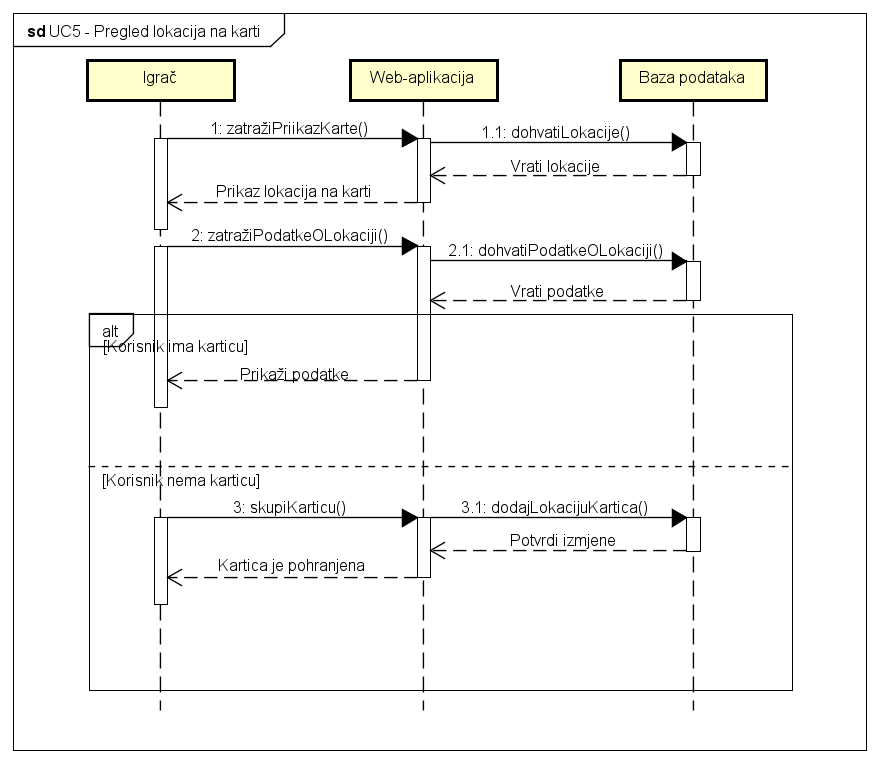
\includegraphics[width=\linewidth, height=14cm]{dijagrami/sd_UC5}
						\centering
						\caption{Sekvencijski dijagram UC5}
						\label{}
					\end{figure}
				\newpage	
				
				\textbf{Obrazac uporabe UC30 - Uređivanje postojeće lokacije}\\
					
					{Kartograf odabire opciju "Prikaz karte". Poslužitelj dohvaća popis lokacija iz baze podataka te ih prikazuje kartografu na karti. Kartograf odabire lokaciju. Poslužitelj dohvaća podatke o lokaciji iz baze podataka te ih prikazuje kartografu.Kartograf šalje zahtjev za promjenu podataka o lokaciji. Poslužitelj mu daje pristup i kartograf unosi nove podatke o željenoj lokaciji. Poslužitelj izmijeni podatke u bazi podataka koja vraća potvrdu.}\\
					
					\begin{figure}[H]
						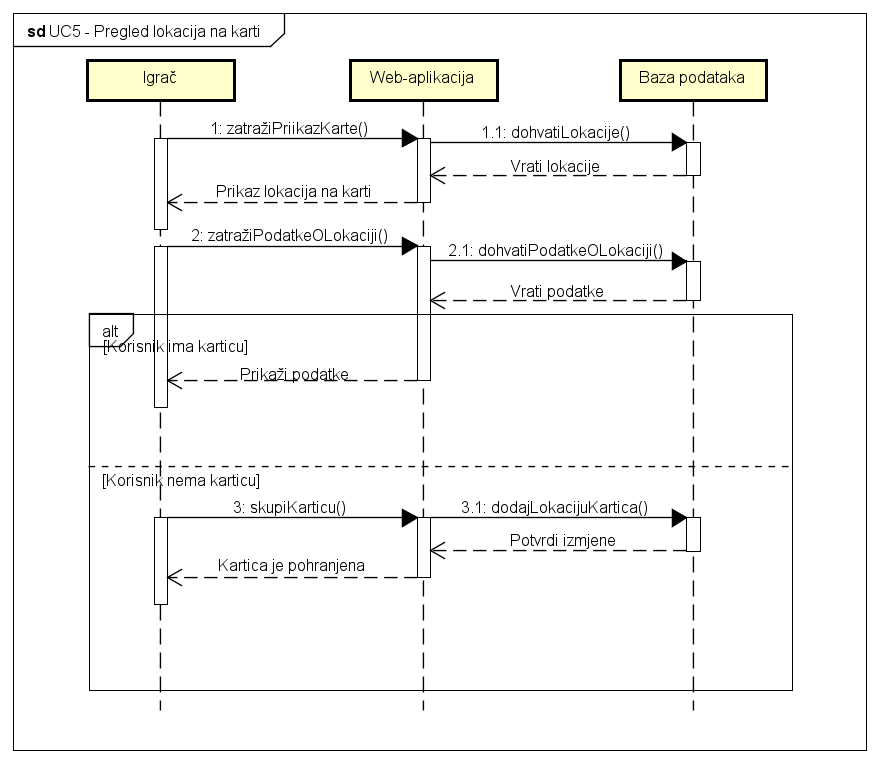
\includegraphics[width=\linewidth, height=14cm]{dijagrami/sd_UC30}				
						\centering
						\caption{Sekvencijski dijagram UC30}
						\label{}
					\end{figure}
					
				
				\eject
	
		\section{Ostali zahtjevi}
		
			\begin{packed_item}
				\item Sustav treba omogućiti rad više korisnika u stvarnom vremenu 
				\item Korisničko sučelje i sustav moraju podržavati hrvatsku abecedu (dijakritičke znakove) pri unosu tekstualnog sadržaja
				\item Izvršavanje dijela programa u kojem se pristupa bazi podataka ne smije trajati duže od nekoliko sekundi
				\item Sustav treba biti implementiran kao web aplikacija koristeći objektno-orijentirane jezike
				\item Neispravno korištenje korisničkog sučelja ne smije narušiti funkcionalnost i rad sustava
				\item Sustav treba biti jednostavan za korištenje, korisnici se moraju znati koristiti sučeljem bez opširnih uputa
				\item Nadogradnja sustava ne smije narušavati postojeće funkcionalnosti sustava
				\item Veza s bazom podataka mora biti kvalitetno zaštićena, brza i otporna na vanjske greške
				\item Pristup sustavu mora biti omogućen iz javne mreže pomoću HTTPS.
			\end{packed_item}
			 
			 
			 
	